\subsection{Probabilistic Payments}
\label{sec:probabilisticpayments}

In traditional payment channels, two parties $A$ and $B$ lock some funds within a
smart contract, make transactions off-chain and only commit the aggregation
on-chain. Thus, a payment channel is bidirectional which means that both $A$ and $B$ can
send and receive transactions within the same payment channel. The HOPR protocol uses
unidirectional payment channels to implement bidirectional payment channel behavior where a
payment channel is created from A to B and another from $B$ to $A$. The payment channel creator is
the sole owner of funds in the payment channel and the one able to create
\textbf{tickets}, encapsulated funds which are described in detail in
\nameref{sec:tickets}. A payment channel created from party $A$ to party $B$ is
different from a payment channel created from party $B$ to party $A$.

$$A\rightarrow B \neq B\rightarrow A$$

This separation reflects the directional nature of packets flowing through the
network. Also each payment channel's logic is easier to verify.

\paragraph{Acknowledgements} are messages which allow every node to acknowledge
the processing of a packet to the previous node. This acknowledgement contains
the cryptographic material to unlock the possible payout for the previous node.
Note that an acknowledgement is always sent to the previous node and using
acknowledgments with vanilla payment channels results in accumulated incentives
where the latest acknowledgement contains all previous incentives plus the
incentive for the most recent interaction as explained below:

\begin{align}
value_(ACK_n) &=\sum_{i=1}^nfee_{packet_i}
\end{align}
where $n$ is the total number of mixnet packets transformed.

An issue arises when $B$ received $ACK_n$ for $packet_n$ before sending
$packet_{n-1}$. At that point $B$ would have no incentive to process
$packet_{n-1}$ rather than $packet_{n}$. To avoid such false incentives the HOPR
protocol utilizes probabilistic payments. A \textit{ticket} can be either a win
or a loss with a winning probability which is lower than 100 percent. This means
nodes are incentivized to continue relaying packets as they don’t know which
ticket is a win and will lead to a payout. To a node each ticket has the same
value untul it is being claimed, thus the HOPR protocol encourages nodes to
claim tickets independently from each other.

\begin{align}
value ( ACK_i )  &  =value ( ACK_j ) \quad for \quad i,j\in \{1,n\}
\end{align}

If we assume the price stays the same, there is no added value in pretending
packet loss or intentionally changing the order in which packets are processed.
On the contrary a node would reduce its potential payouts when not forwarding
packets as fast as possible or not at all.

\subsection{Payment Channel Management}
\label{sec:paymentchannelmanagement}

Initially, each payment channel is \textit{Closed}. For node $A$ to be able to
transfer packets to node $B$ it has to open a payment channel first. There are
four distinct payment channel states which are represented in the following
scheme:

\begin{figure}[H]
    \centering
    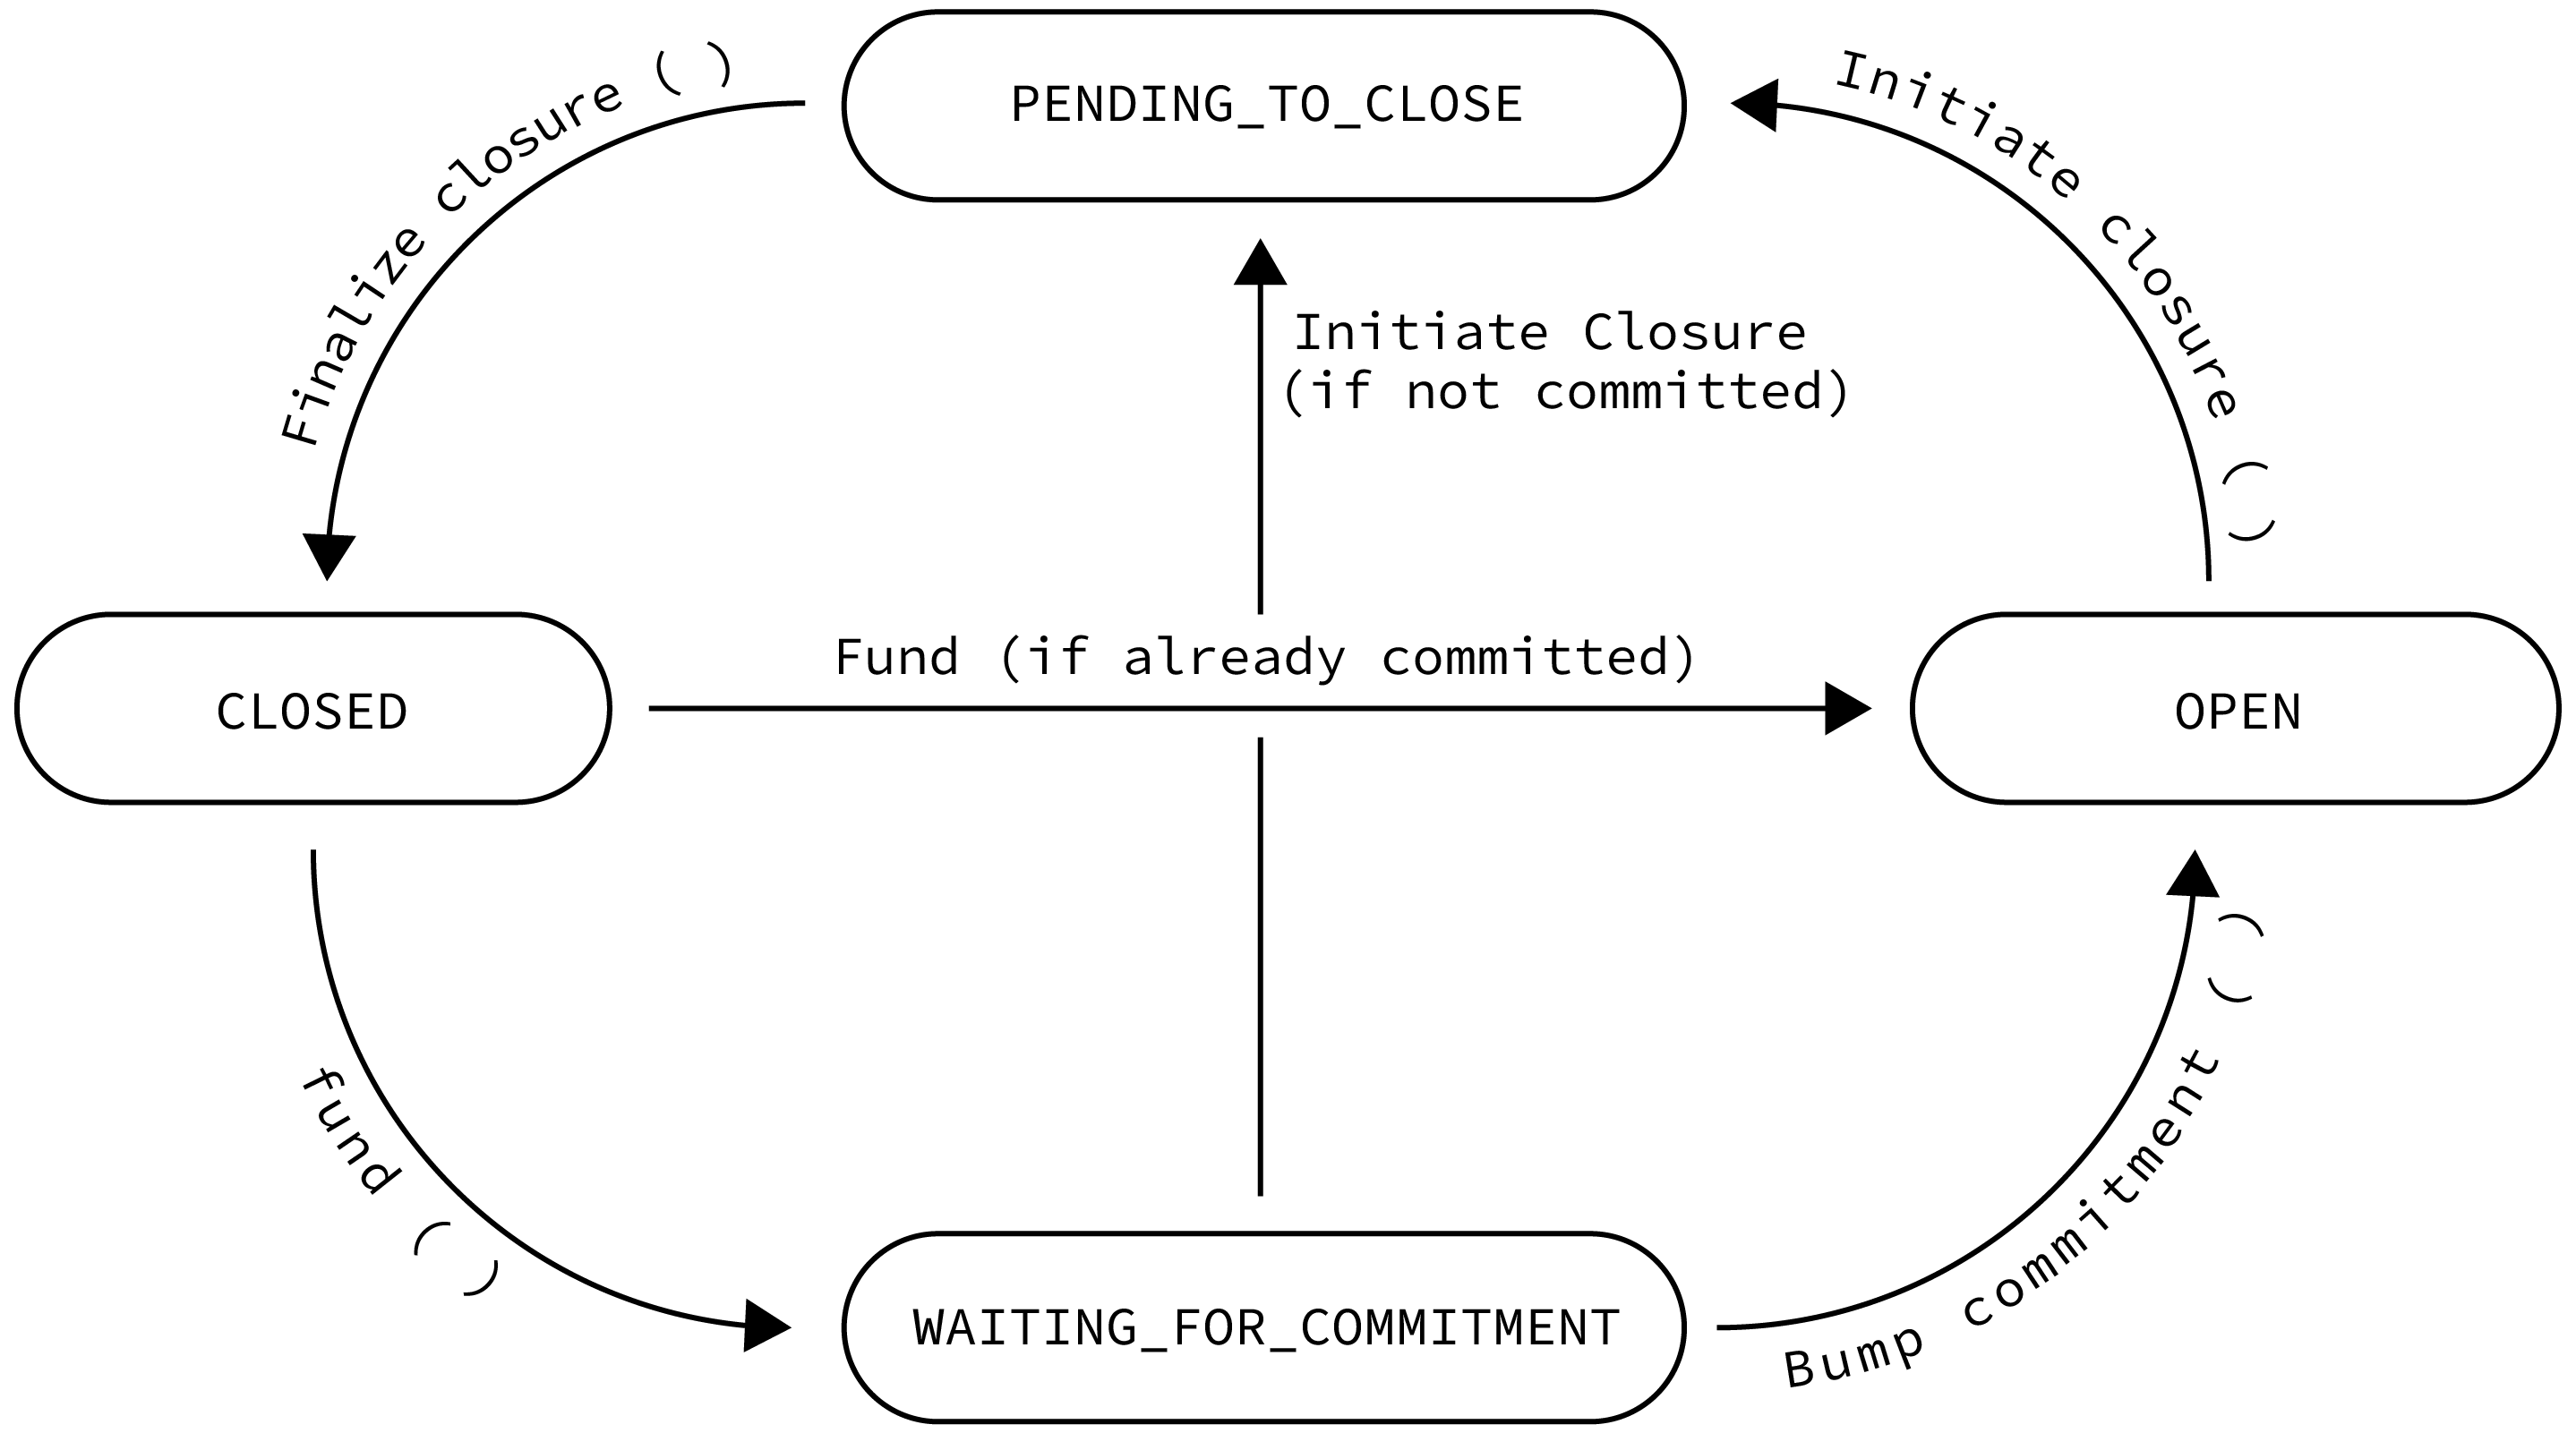
\includegraphics[width=9cm,height=9cm,keepaspectratio]{../yellowpaper/images/statesTransition.png}
    \label{fig:payment channel states}
    \caption{Payment channel states}
\end{figure}

\paragraph{Opening a channel} can be done by node $A$ by transferring funds to
the payment channels contract \textit{HoprChannels} and include the following
\textit{userdata}:

$$[A: address, B: address, \lambda: uint8, \mu: uint8], \mu = 0$$

$\lambda$ is the amount to be staked by the sender $A$. This will open a
unidirectional payment channel from $A$ to $B$. The payment channel will start
in state \textit{Waiting for commitment}. The destination address $B$ of the
payment channel must now set an on-chain commitment in order for the payment
channel between both parties to become \textit{Open}. This is done by $B$
calling the \textit{bumpChannel()} function to make a new set of commitments
towards this payment channel. This call will trigger an on-chain event
\textit{ChannelIsOpened} and bumps the ticket epoch to ensure tickets with the
previous epochs are invalidated.

\paragraph{Redeem tickets}
As long as the channel remains open, nodes can claim their incentives for
forwarding packets via tickets. Tickets are redeemed by dispatching a
\textit{redeemTicket()} call to an \textit{Open} payment channel.

When $B$ tries to redeem a ticket from the channel $A\rightarrow B$ (spending
channel) but also there is an open channel $B\rightarrow A$ (earning channel),
$B$'s rewards will be transferred to $B\rightarrow A$ (earning channel).
Otherwise, rewards will be sent directly to $B$.

\paragraph{Closing a channel}
Nodes can close a payment channel in order to access their previously staked
funds. Only the payment channel creator can initiate the process by calling
\textit{initiateChannelClosure()}. This changes the state to $Pending to close$
which is a limited timeframe (grace period) during which other nodes can redeem
so far unredeemed tickets. Therefore, nodes should monitor blockchain events to
be aware of this payment channel state change.
Once the timeframe has completed, the payment channel creator can call
\textit{finalizeChannelClosure()} which turns the payment channel state into
$Closed$. When a payment channel is closed, funds (stake) are transfered
automatically back to the payment channel creator. Every ticket that wasn't
redeemed while payment channel was open can not be redeemed after closure. This
is guaranteed by using a channel epoch.

\begin{comment}

\begin{figure}[H]
    \centering
    \begin{tikzpicture}[looseness=1,auto]
        \path (0,0) node (closed) [ellipse,draw] {$Closed$};
        \path (-1,-1)  node (commitment) [ellipse,draw,align=left] {$Waiting$\\$Commitment$};
        \path (5,0)  node (open) [ellipse,draw] {$Open$};
        \path (2.5,-1)  node (pending) [ellipse,draw,align=left] {$Pending$\\$Timeout$};

        \draw [->,draw](closed) to [bend left] node {\textsf{fund()}} (commitment);
        \draw [->,draw](commitment) to [bend left] node {\textsf{fund()}} (open);
        \draw [->,draw](open) to [bend left] node [align=center] {\textsf{initiateChannelClosure()}} (pending);
        \draw [->,draw](pending) to [bend left] node {\textsf{finalizeChannelClosure()}} (closed);

        \path[->] (open) edge [out=+120,in=+60,distance=2em,below] node [align=center,above] {\textsf{redeemTicket()}}  (open);
    \end{tikzpicture}
    \label{fig:channel workflow}
    \caption{Channel workflow}
\end{figure}
\end{comment}

\begin{comment}
  \draw [->,draw](commitment) to [bend left] node {\textsf{fund()}} (open);
    \draw [->,draw](open) to [bend left] node [align=center] {\textsf{initiateChannelClosure()}} (pending);
    \draw [->,draw](pending) to [bend left] node {\textsf{finalizeChannelClosure()}} (closed);  
\end{comment}
